\begin{frame}
	\frametitle{Generación del escenario}
	
	\begin{columns}
		\column{0.6\textwidth}
		\begin{itemize}
			\item<1-> Se divide el mapa en \textcolor{UDCpink}{islas}.
			\vspace{0.5em}
			
			\begin{enumerate}
				\item<2-> Se define que regiones cuentan para una isla.
				\vspace{0.5em}
				\item<3-> Se detalla el contorno de la isla.
			\end{enumerate}
		
			\vspace{0.5em}
			\item<4-> Los módulos son \textcolor{UDCpink}{independientes}. No necesitan toda la información del problema.
		\end{itemize}
		
		\column{0.4\textwidth}
		\centering
		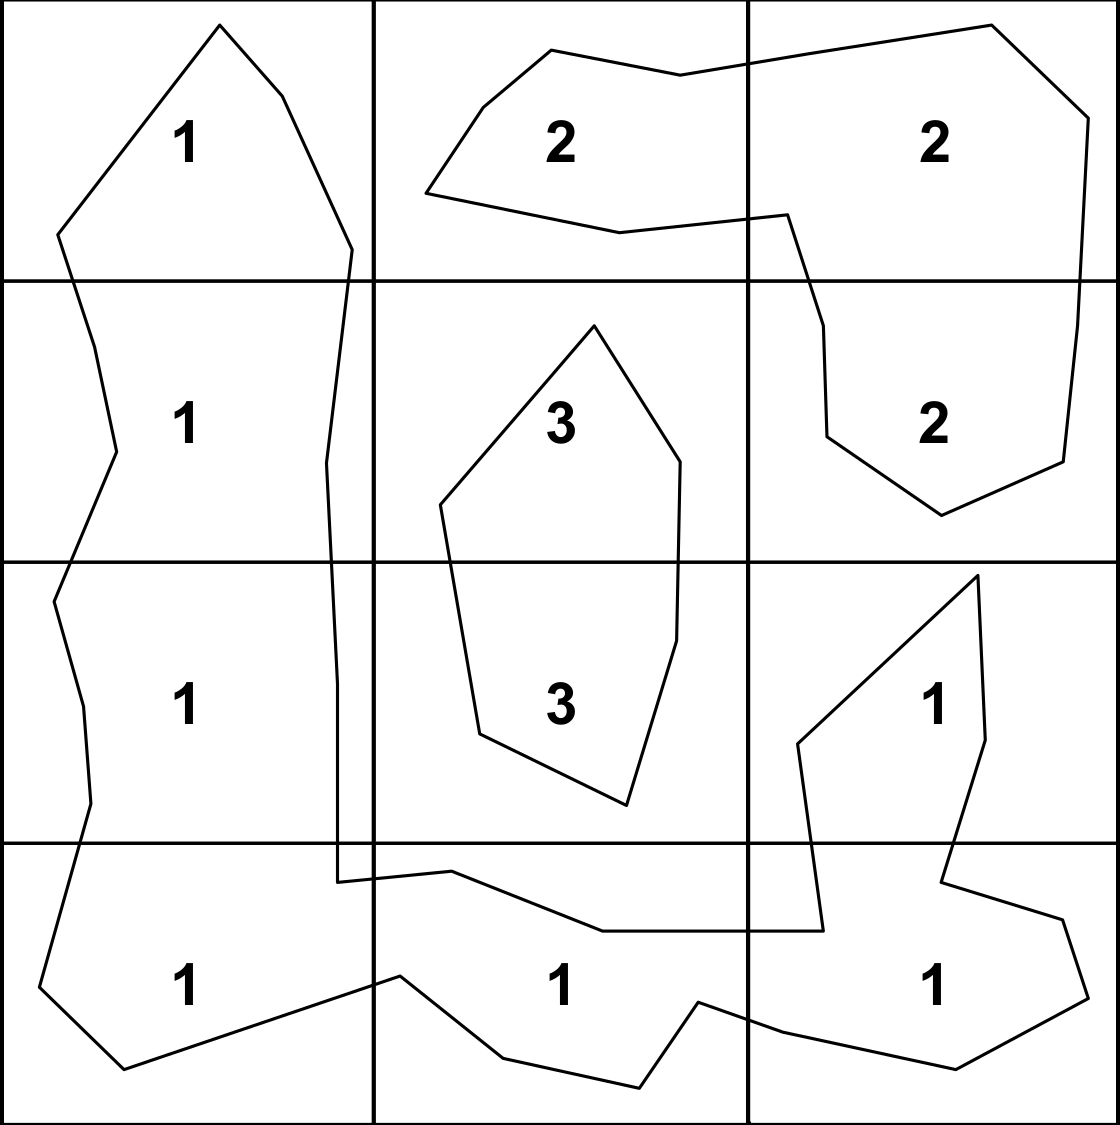
\includegraphics[width=0.8\textwidth]{images/regiones.png}
	\end{columns}
\end{frame}

\begin{frame}
	\frametitle{Generación de biomas y de puntos de inicio}
	
	\begin{columns}
		\column{0.6\textwidth}
		
		\begin{itemize}
			\item<1-> \textcolor{UDCpink}{Generación de biomas}:
			
			\vspace{0.5em}
			
			\begin{itemize}
				\item<1-> Un bioma es una zona con el \textcolor{UDCpink}{mismo tipo de terreno}.
				
				\vspace{0.5em}
				
				\item<2-> Misma forma que la generación de islas, salvo que se pueden \textcolor{UDCpink}{pegar}.
			\end{itemize}
		\end{itemize}
		
		\column{0.4\textwidth}
		\centering
		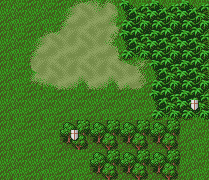
\includegraphics[width=0.6\textwidth]{images/biomas.png}
		
	\end{columns}
	
	\vspace{1em}
	
	\begin{itemize}
		\item<3-> \textcolor{UDCpink}{Generación de puntos de inicio}:
		
		\vspace{0.5em}
		
		\begin{itemize}
			\item<3-> Se escoge N celdas de tierra para los jugadores.
			
			\vspace{0.5em}
			
			\item<4-> Para estos puntos se añaden preferencias:
			
			\vspace{0.5em}
			\begin{itemize}
				\item<4-> \textcolor{UDCpink}{Minimizar la distancia al agua}.
				
				\vspace{0.5em}
				
				\item<5-> \textcolor{UDCpink}{Maximizar la distancia a las montañas}.
			\end{itemize}
		\end{itemize}
	\end{itemize}

\end{frame}